\documentclass{beamer}
\usetheme{metropolis}           % Use metropolis theme
\usepackage[utf8]{inputenc}
%\usepackage[brazil]{babel}
\usepackage[normalem]{ulem}
\usepackage{float}
\usepackage{caption}
\usepackage{subcaption}
\usepackage{graphicx}
\usepackage{xcolor}
\usepackage[backend = biber]{biblatex}
%\addbibresource{refs.bib}
\metroset{background=light}
\addbibresource{refs.bib}
\usepackage{tikz}
\def\checkmark{\tikz\fill[scale=0.4](0,.35) -- (.25,0) -- (1,.7) -- (.25,.15) -- cycle;}
\title{Majoritarian principles in critical junctures: an analysis of Brazil's
  2018 presidential election}

\date{}
\author{Marcelo Veloso Maciel}
\institute{University of California, Irvine}
\begin{document}
\maketitle

% ----------------- NOVO SLIDE --------------------------------
\begin{frame}
\frametitle{Rationale: highly divisive candidates}
  \begin{figure}[H] \centering 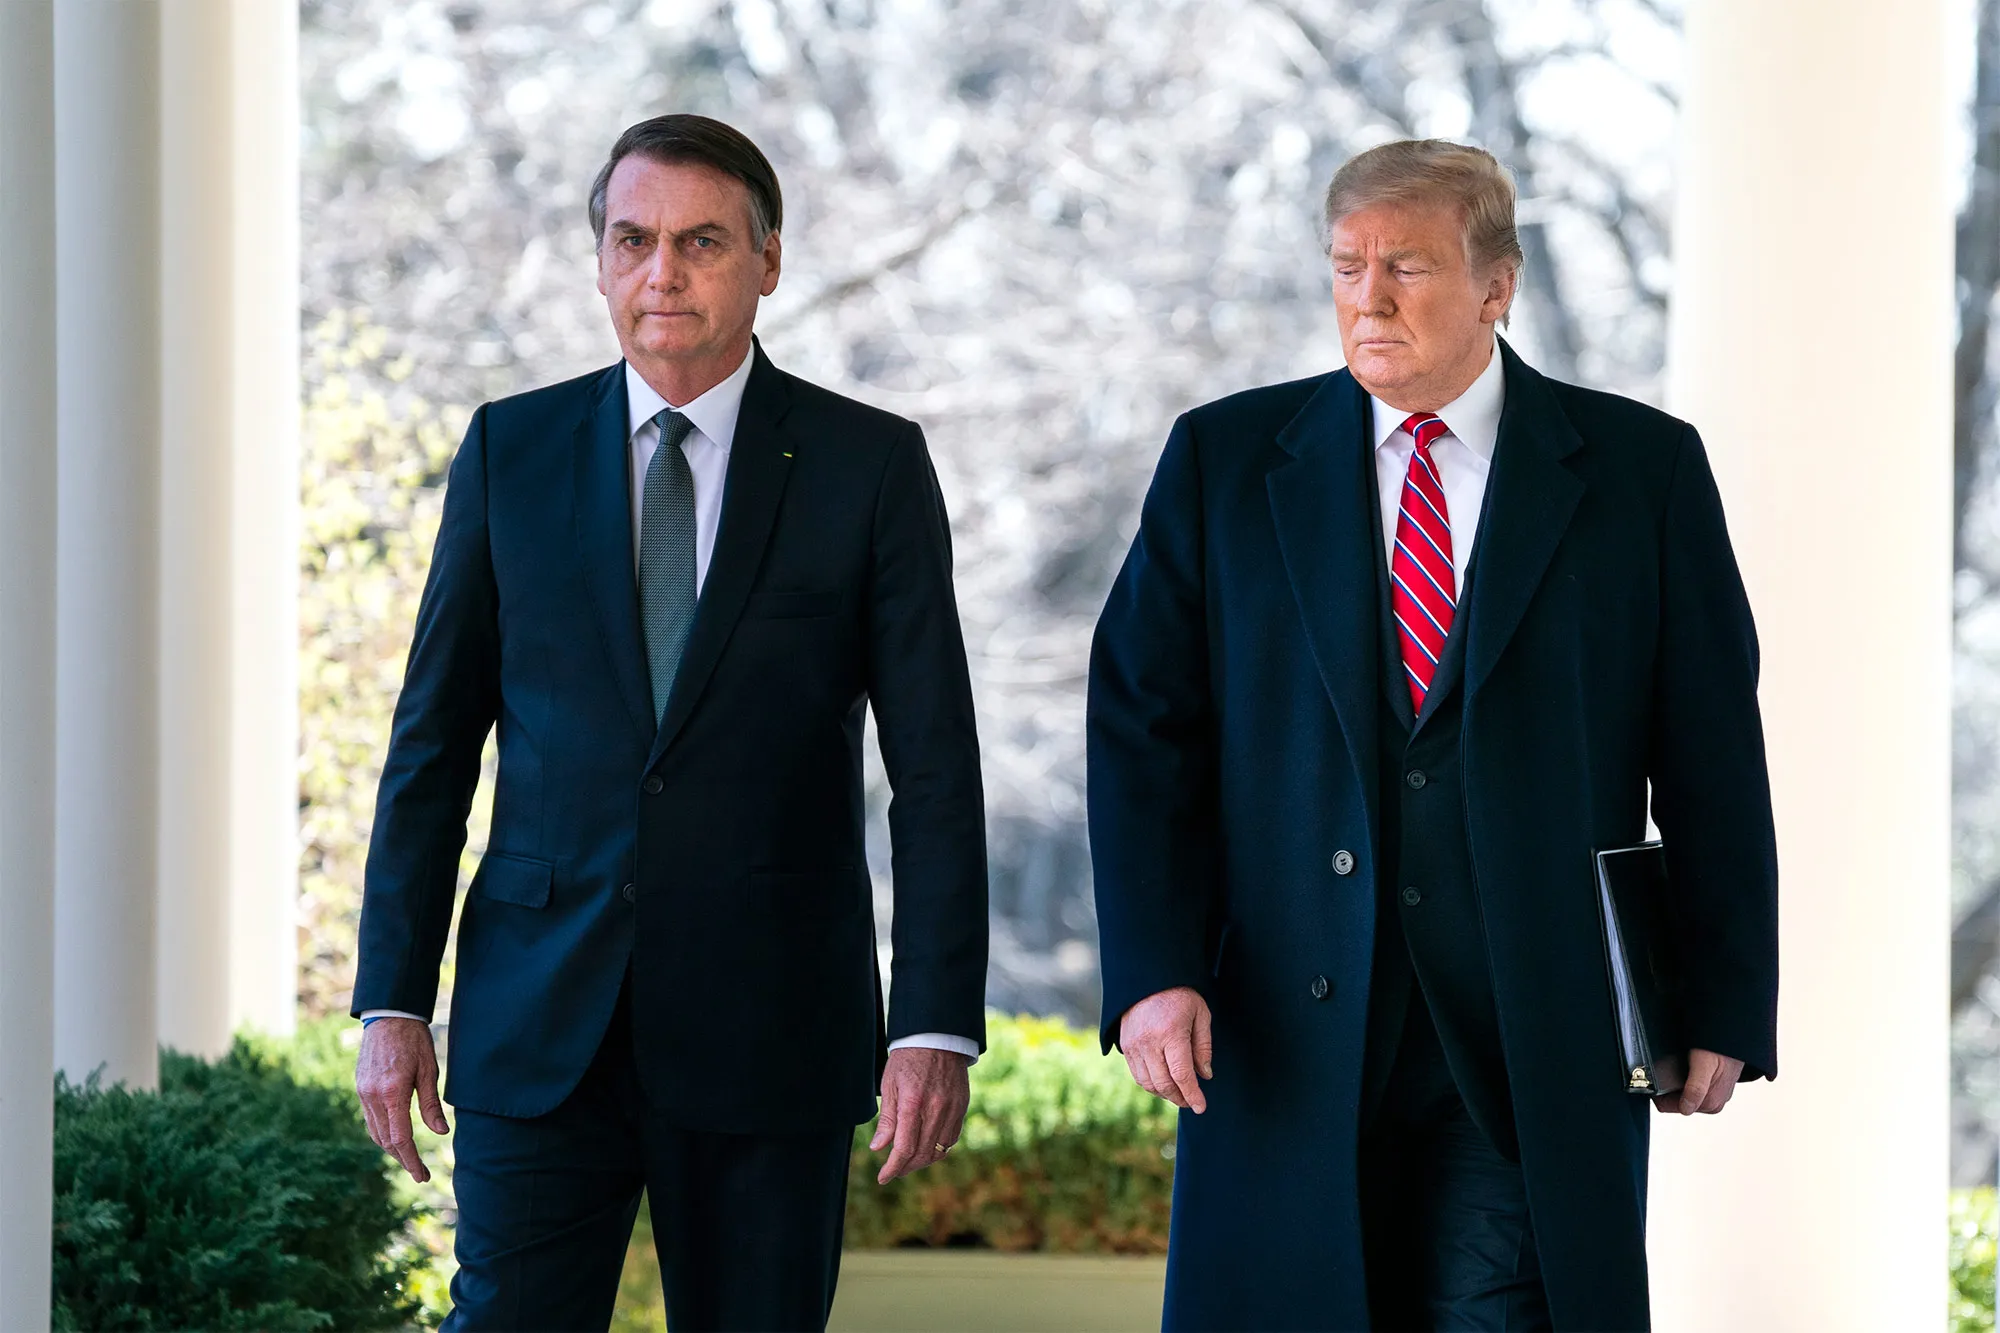
\includegraphics[width=\textwidth]{./trumpolnaro.png}
 %\caption{Jair Messias Bolsonaro and Donald Trump}
 \end{figure}
\end{frame}

\begin{frame}
  \frametitle{Research Question }
  Is the election of divisive or polarizing candidates an artifact of the voting
  methods?
\end{frame}

\begin{frame}
  \frametitle{Prior research}
  \begin{itemize}
    \item \textcite{potthoff2021condorcet} and \textcite{kurrild2018trump} argue
          that Trump might have been a Condorcet loser. \textcite{woon2020trump}
          argue he was in the Core.
    \item \textcite{igersheim22_compar_votin_method} argue that the Condorcet,Borda,Utilitarian winner was actually Sanders.
  \end{itemize}
\end{frame}

\begin{frame}
  \frametitle{Argument/Expectations/Hypotheses}
  \begin{itemize}
    \item I expected similar results in the Brazilian 2018 presidential
          elections. Particularly, I expected him to have neither ``pairwise''
          nor high ``positional'' mandate;
    \item The reason: high rejection would be taken into account by voting
          procedures that use the whole ranking. Information paucity would be
          causing the electoral victory of divisive candidates.
  \end{itemize}
\end{frame}


\begin{frame}
  \frametitle{Data and Method }
  \begin{itemize}
    \item I use a ``representative'' street survey a week before the first round of the presidential election. A pairwise comparison of the top 4 candidates was the only question I analyzed.
    \item Not all respondents compared all candidates. I imputed the data with a
          polytomous regression\footnote{Using the \textbf{\textsf{R}} package
          \(\operatorname{mice}\)}.
    \item There was a discrepancy between the survey and the result of the first
          round. I transferred while respecting Kemeny's distance, and picked
          the transferrence with minimal euclidean distance to the result.
  \end{itemize}
\end{frame}

\begin{frame}
  \frametitle{Method - Saari's Outcome Triangle}
\begin{figure}[H] \centering 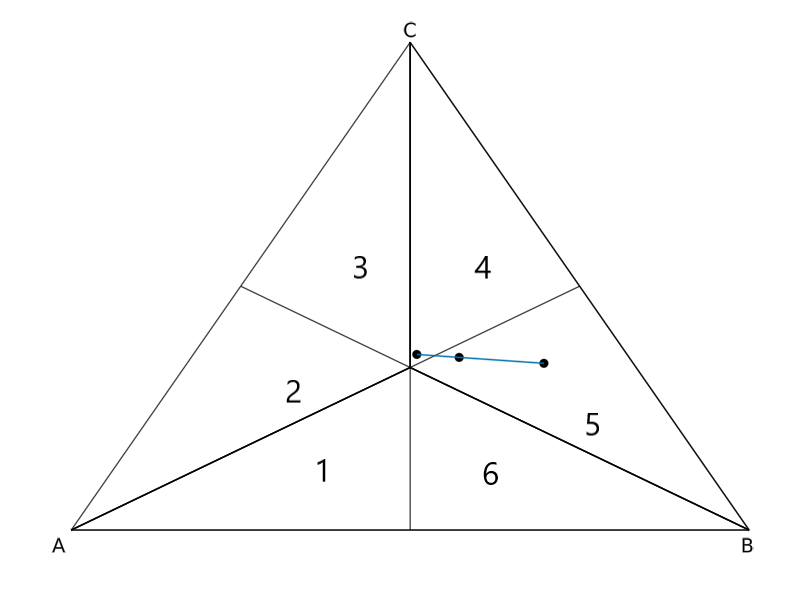
\includegraphics[width=\textwidth]{../images/simpletriangle.png}
 \caption{Saari's outcome simplex}
 \label{fig:saari_nurmi}
\end{figure}
\end{frame}


\begin{frame}
  \frametitle{Profile after imputation and rankings transference}
\begin{figure}[!h] \centering
  \begin{subfigure}[b]{0.49\textwidth} \centering
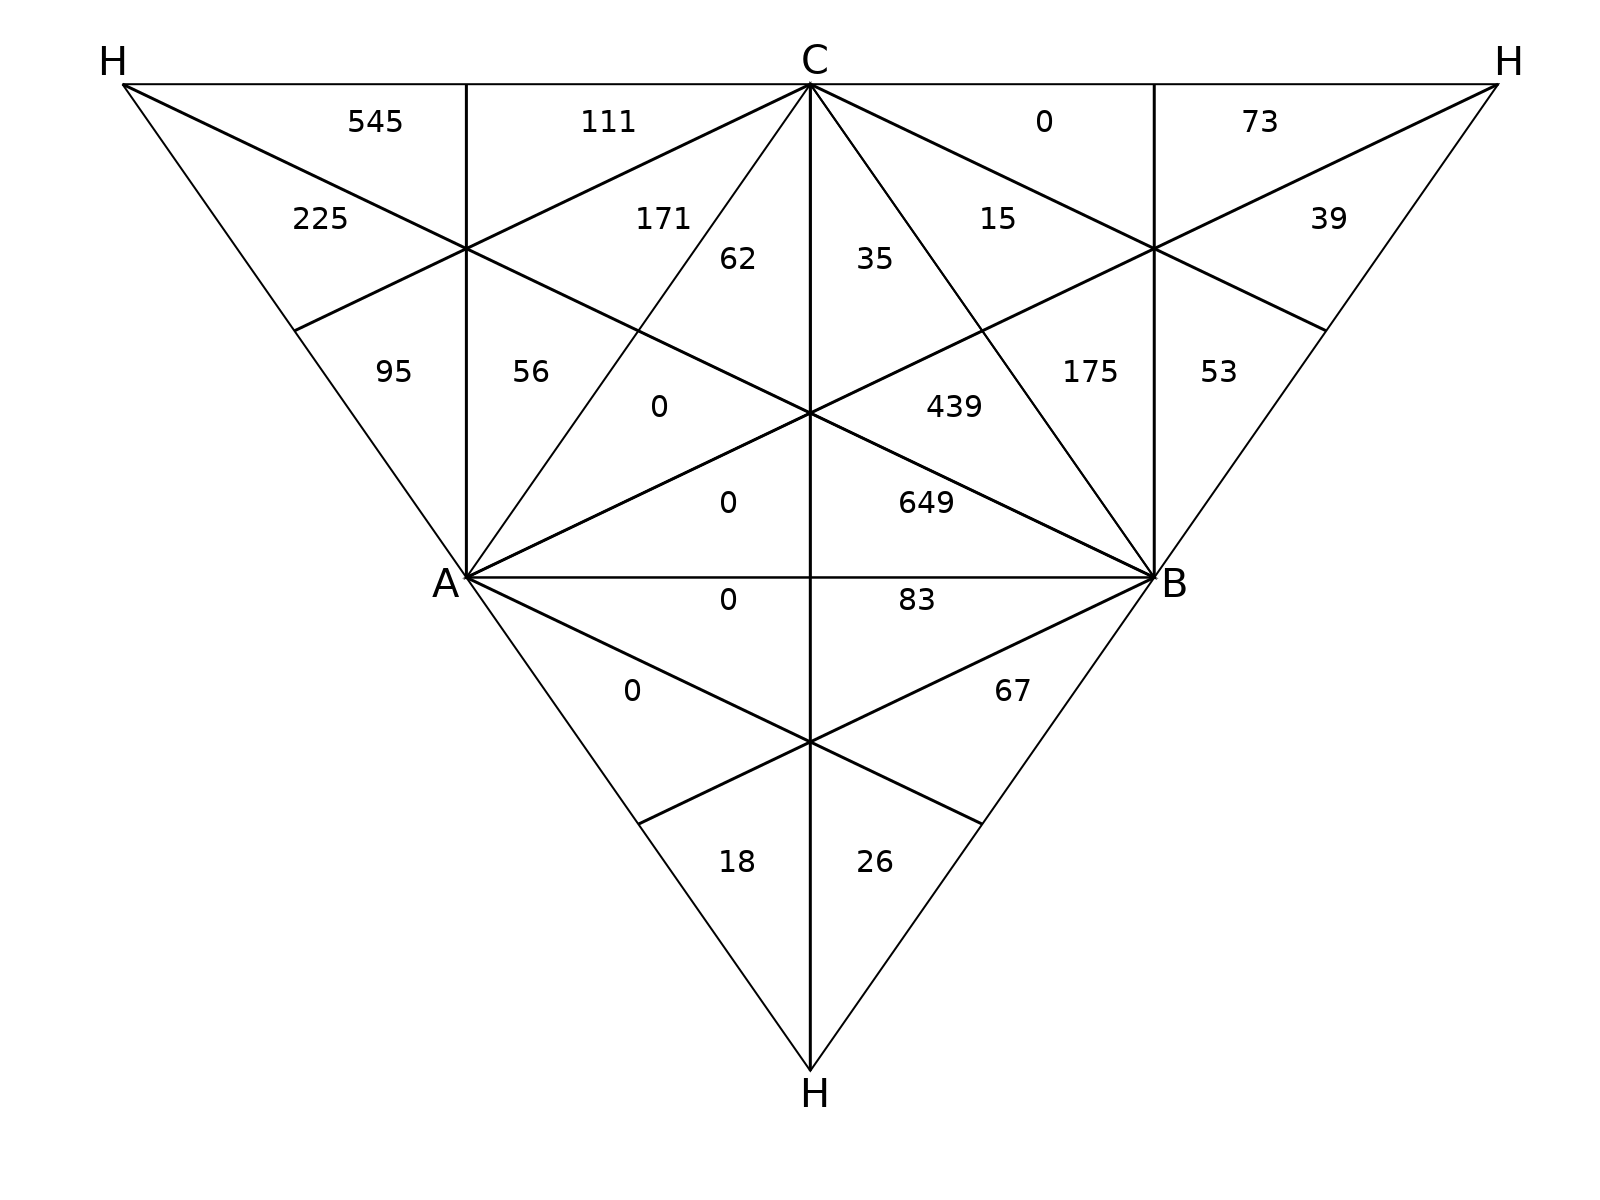
\includegraphics[width=\textwidth]{../images/representation_tetrahedron.png}
 \caption{Opened representation tetrahedron}
 \label{fig:rep_ot}
\end{subfigure} \hfill
  \begin{subfigure}[b]{0.49\textwidth} \centering
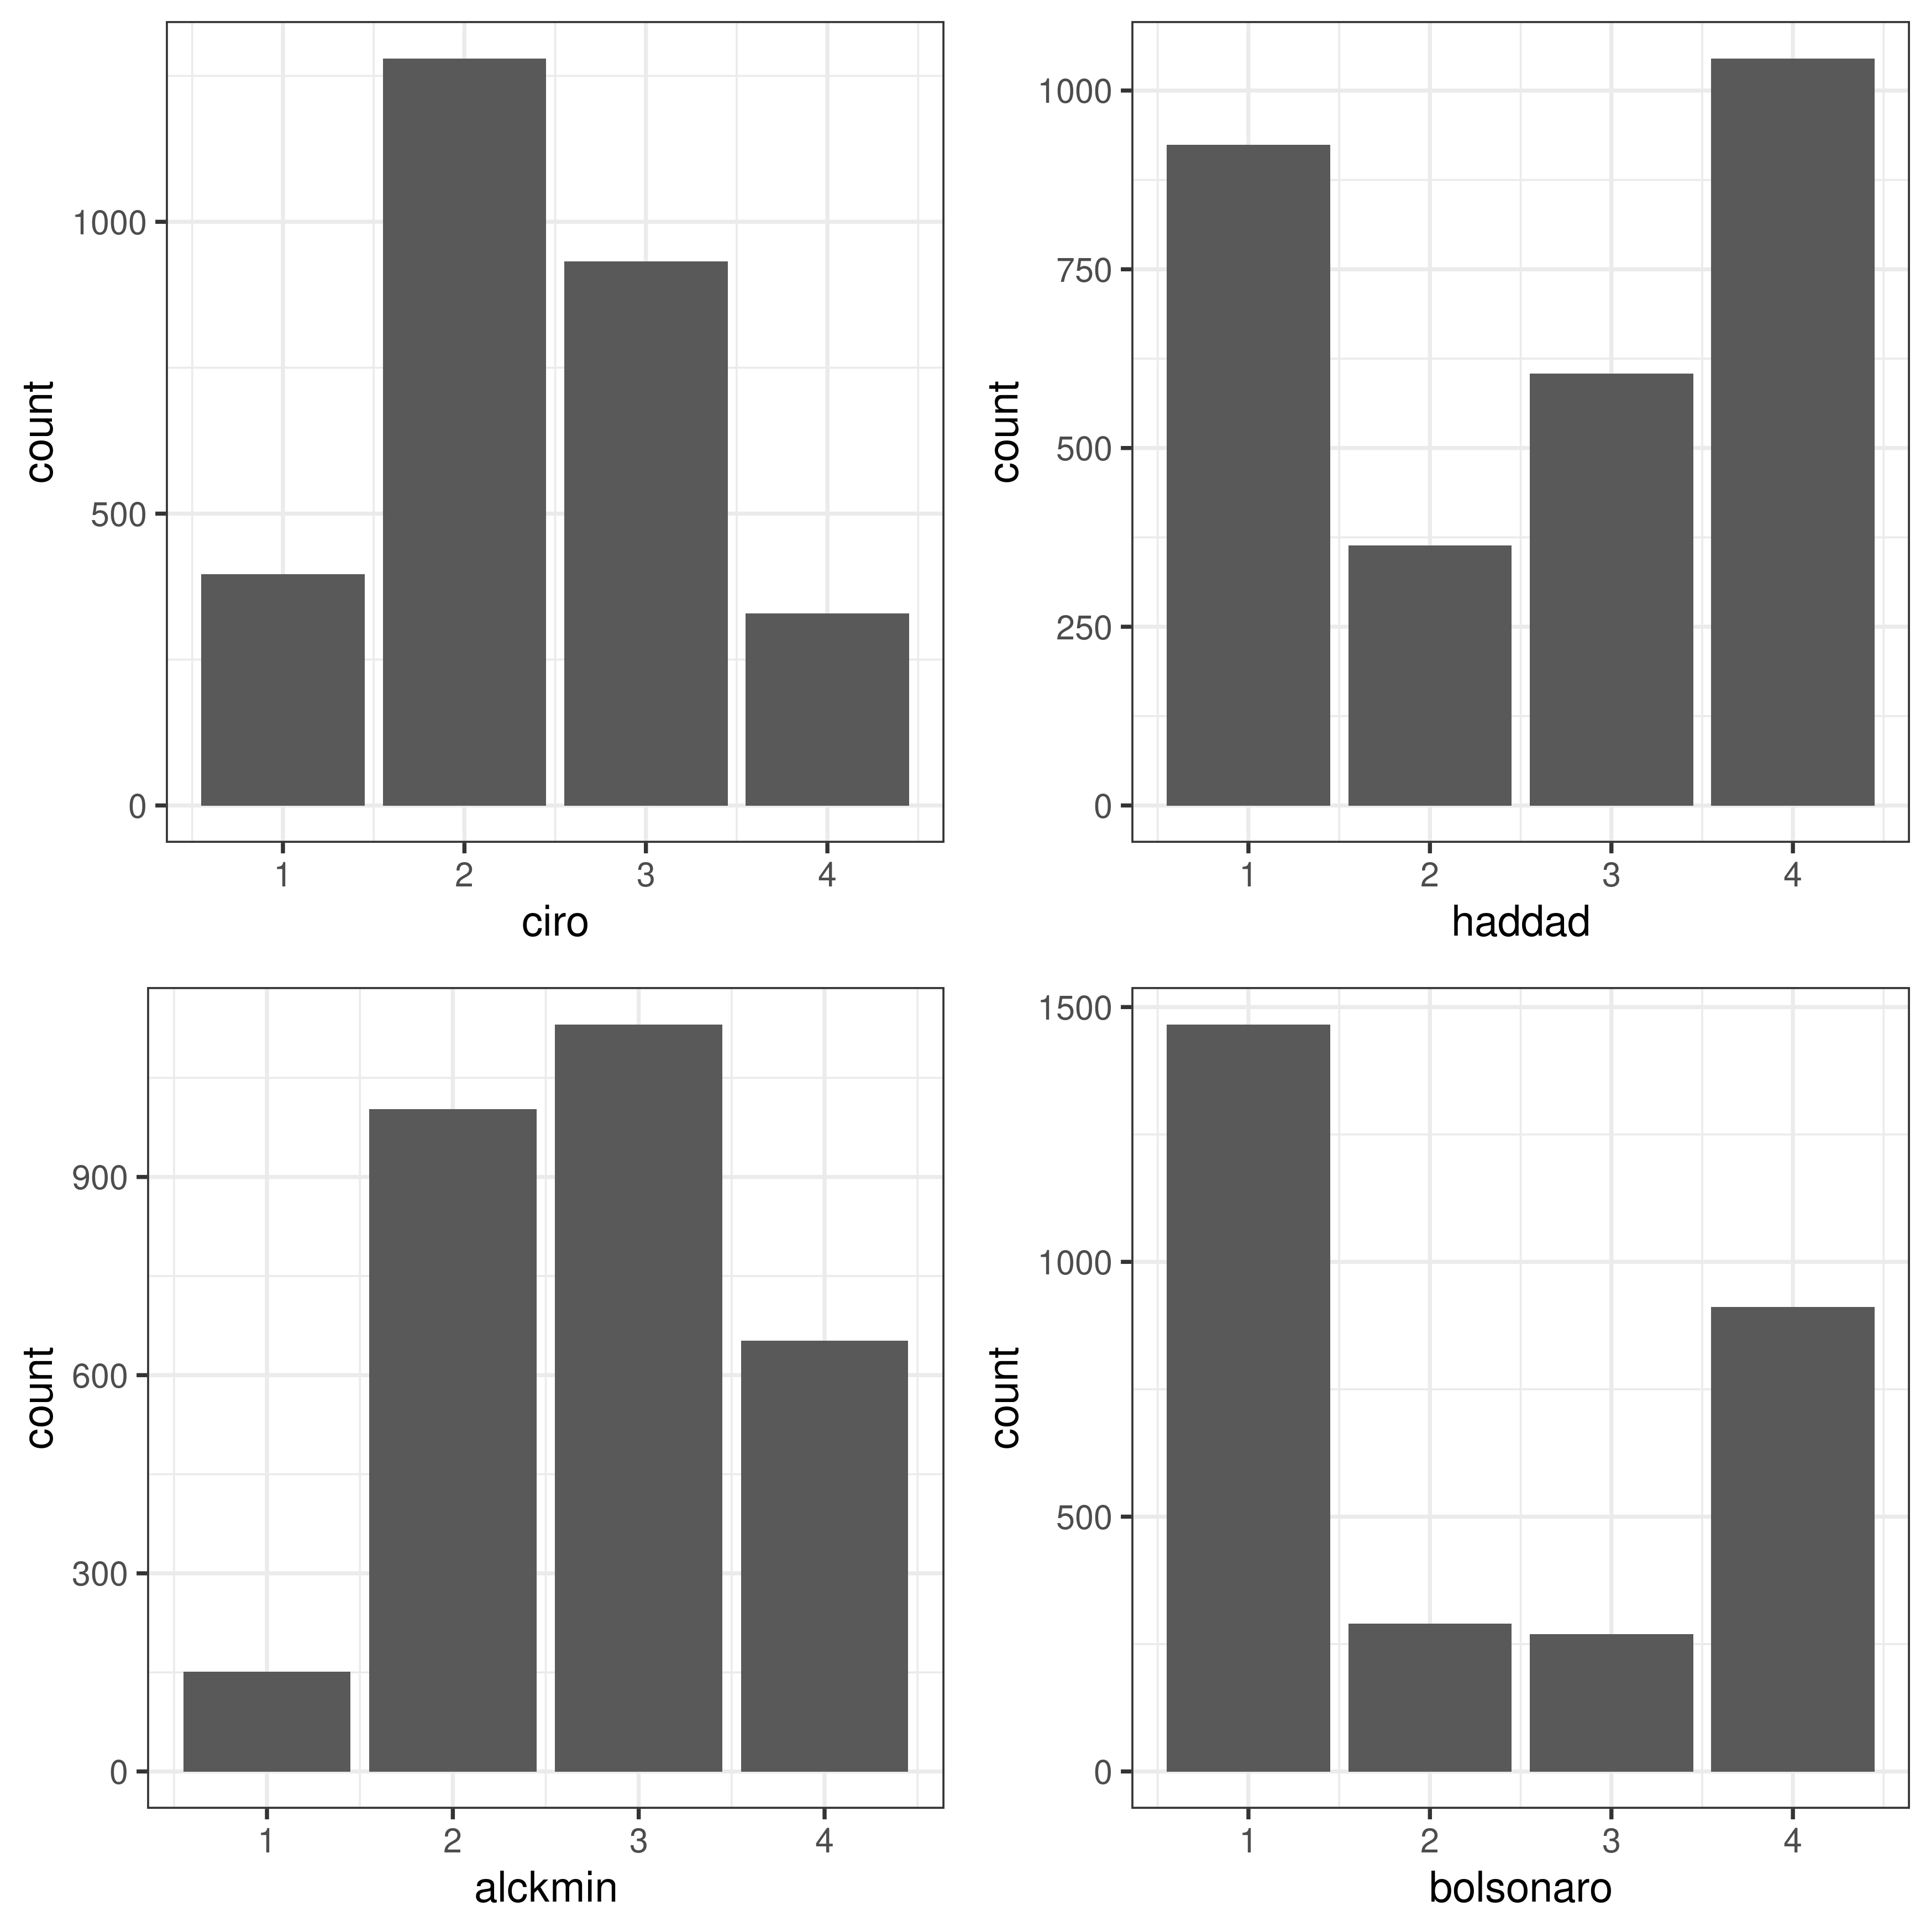
\includegraphics[width=\textwidth]{../images/corrected1_indexes_plot.png}
 \caption{Frequencies at each position}
 \label{fig:counts}
\end{subfigure}

\end{figure}
\end{frame}

\begin{frame}
  \frametitle{Results I: Borda and Condorcet}

\begin{table}[!h]
\centering
\begin{tabular}{rrrrr} & Alckmin & Bolsonaro & Ciro & Haddad \\\hline Alckmin &
  0.0\% & -12.63\% & -16.99\% & 8.27\% \\ Bolsonaro & 12.63\% & 0.0\% & 5.48\% &
  7.46\% \\ Ciro & 16.99\% & -5.48\% & 0.0\% & 16.65\% \\ Haddad & -8.27\% &
  -7.46\% & -16.65\% & 0.0\% \\\hline
          \end{tabular}
          \quad

\begin{tabular}{rrr} \hline & Borda Score & Standardized Borda Score\\ \hline
  Alckmin & 7029 & 0.464 \\ Bolsonaro & 7718 & 0.543 \\ Ciro & 7756 & 0.547\\
  Haddad & 6867 & 0.446 \\ \hline
\end{tabular}
\end{table}

\end{frame}

\begin{frame}
  \frametitle{Opened Tetrahedron - Four candidates Positional Result}
\begin{figure}[!h] \centering 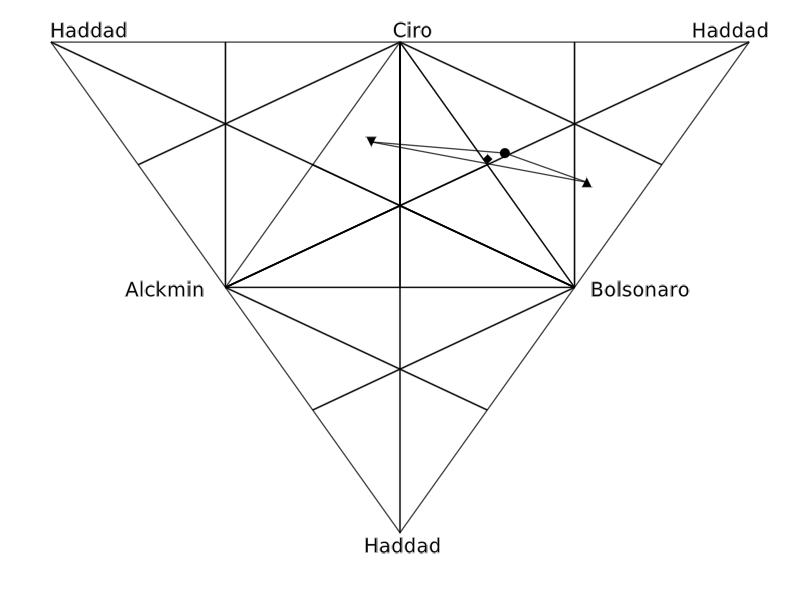
\includegraphics[width=\textwidth]{../images/opened_tetrahedron1.png}
 %\caption{Saari's opened tetrahedron }
 
\end{figure}

\end{frame}

\begin{frame}
  \frametitle{Counterfactual Positional Victories }
\begin{table}[H]
  \centering
  \begin{tabular}{rrrrr}
    \hline
     & Alckmin & Bolsonaro & Ciro & Haddad \\
    \hline
    Alckmin & 0.0 & 0.31 & 0.0 & 0.58 \\
    Bolsonaro & 0.69 & 0.0 & 0.47 & 1.0 \\
    Ciro & 1.0 & 0.53 & 0.0 & 0.81 \\
    Haddad & 0.42 & 0.0 & 0.19 & 0.0 \\\hline\hline
  \end{tabular}
  % \caption{Proportion of victories in the positional voting procedure set}
  \label{tbl:ctn}
\end{table}

\end{frame}

\begin{frame}
  \frametitle{Victory in terms of \(s_1\) and \(s_2\)}
\begin{figure}[!h] \centering 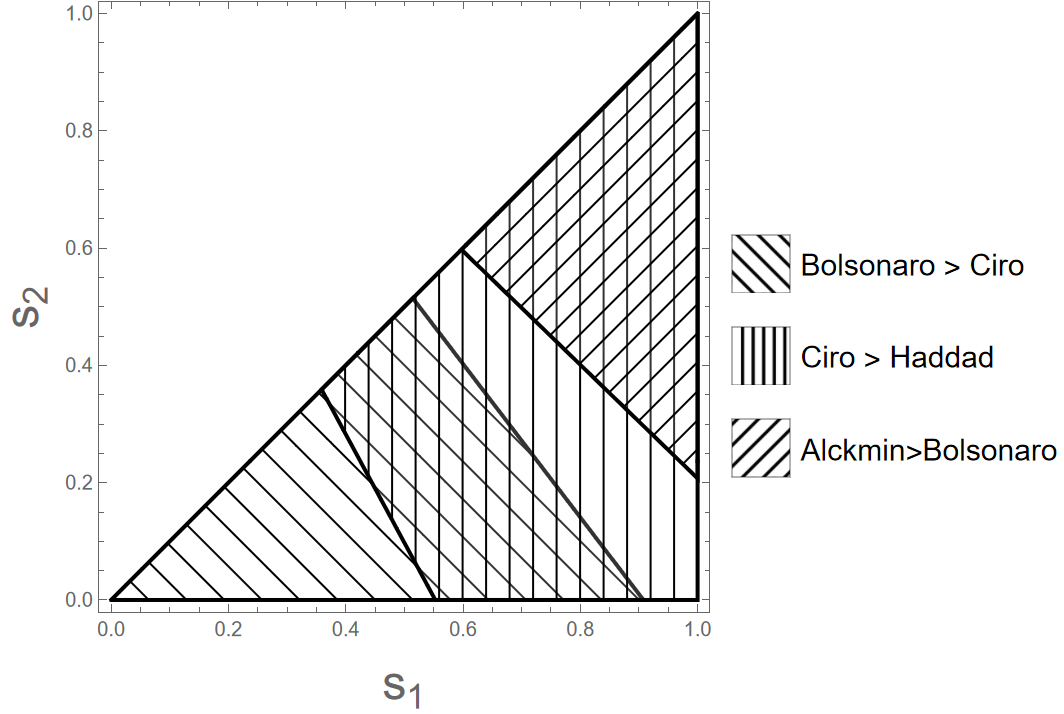
\includegraphics[width=\columnwidth]{../images/counterfactual_triangle.png}
\end{figure}


\end{frame}

\begin{frame}
  \frametitle{Alternative Set Stability }

   \begin{figure}[!h] \centering
        \begin{subfigure}[b]{0.45\textwidth} \centering
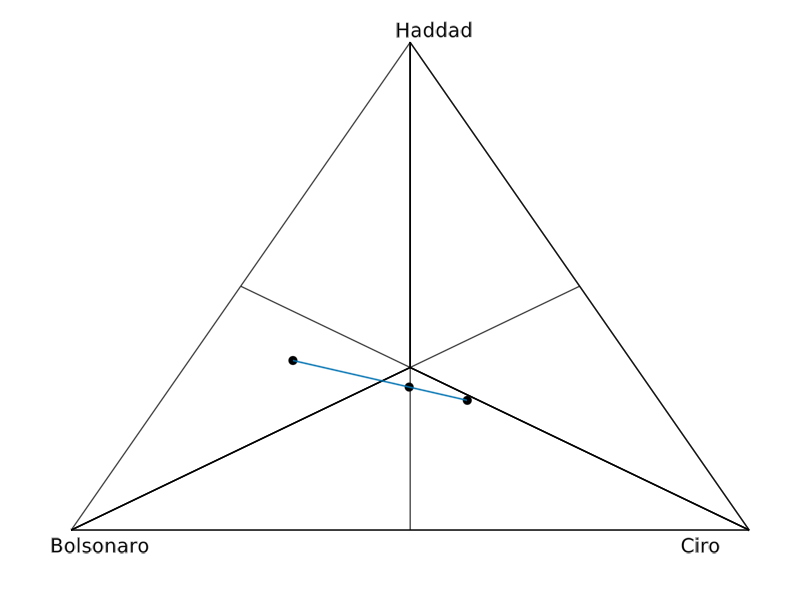
\includegraphics[width=\textwidth]{../images/cw1_nota.png}

        \end{subfigure} \hfill
        \begin{subfigure}[b]{0.45\textwidth} \centering
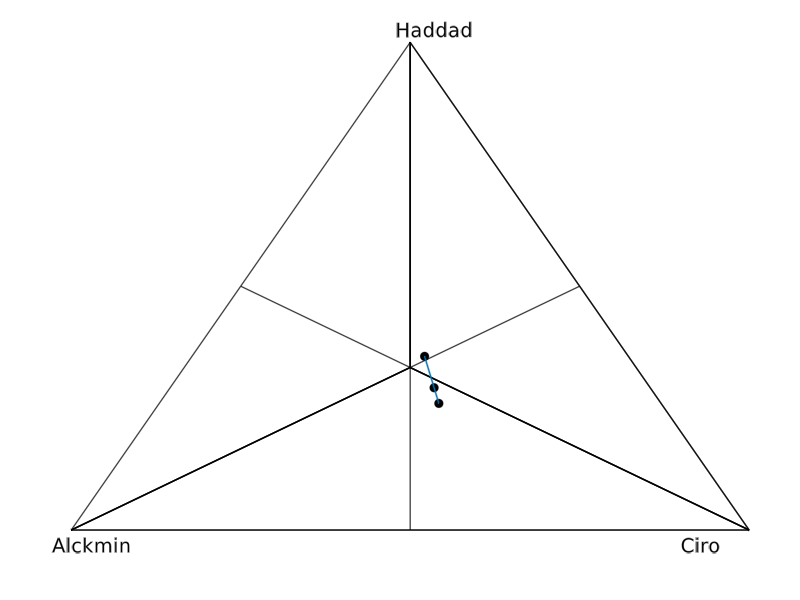
\includegraphics[width=\textwidth]{../images/cw1_notb.png}

        \end{subfigure} \vskip\baselineskip
        \begin{subfigure}[b]{0.45\textwidth} \centering
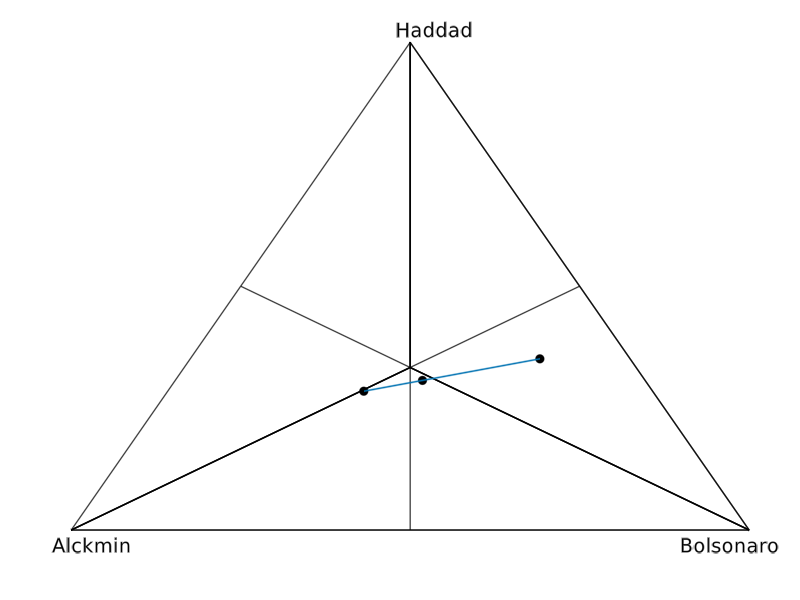
\includegraphics[width=\textwidth]{../images/cw1_notc.png}

        \end{subfigure} \hfill
        \begin{subfigure}[b]{0.45\textwidth} \centering
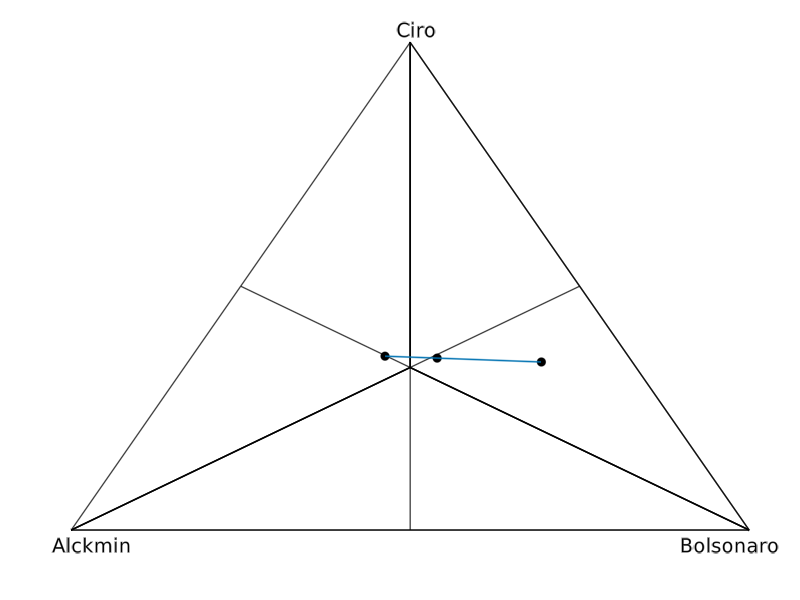
\includegraphics[width=\textwidth]{../images/cw1_noth.png}
        \end{subfigure}
        \caption[ Positional results when dropping one candidate ] {\small
Positional results after dropping one candidate }
        \label{fig:c1dropping}
    \end{figure}

\end{frame}

\begin{frame}
  \frametitle{Discussion}
  \begin{itemize}
    \item We can't conclude Bolsonaro's victory was an institutional fluke.
          However, there is a conflict between the visions of Condorcet and
          Borda in this case.
    \item They perfectly match had he not ran.
  \end{itemize}
\end{frame}

\begin{frame}
  \frametitle{Conclusion}
  \begin{itemize}
    \item Even though the aggregation procedure boosted Bolsonaro's victory, it was not merely its effect, contrary to established theoretical expectations;
    \item But neither was he an undisputed winner:
    \begin{itemize}
      \item pairwise mandate: \textcolor{green}{\checkmark}
      \item positional mandate: \textcolor{red}{\(\times\)}
    \end{itemize}
  \end{itemize}
\end{frame}

\begin{frame}
  \frametitle{Conclusion}
   Next steps:
    \begin{itemize}
      \item Use other variables in the dataset, particularly in the imputation;
      \item Analyze other moments of the 2018 election;
      \item Simulate coalitional and strategic alternative scenarios;
    \end{itemize}
\end{frame}

\frame[allowframebreaks]{

\tiny\printbibliography
}

  \end{document}


%% \section*{Referências}
%% \begin{frame}[allowframebreaks]{Referências}
%% \printbibliography[heading=none]
%% \end{frame}


%%% Local Variables:
%%% mode: latex
%%% TeX-master: ""
%%% End:
